\chapter{Auswertung der Performancetests}
In diesem Kapitel werden die Performancetests, die mit Apache JMeter mit den jeweiligen Testplänen durchgeführt wurden, ausgewertet. Es wurden drei Testpläne durchgeführt, Lasttest, Skalierbarkeitstest sowie der Stresstest und zu jedem Test folgt eine Auswertung. Diese Auswertung wird vergleichend betrachtet, da es zwei Ressource Server gibt, auf denen die Tests jeweils angewandt wurden, nämlich einmal der Ressource Server, der die Zugriffskontrolle mit Open Policy Agent entkoppelt und der zweite Ressource Server, der die Zugriffskontrolle in dem Server selbst implementiert. Der HTML-Report, der von Apache JMeter aus den Messwerten in der csv-Datei erstellt wird, gibt eine Reihe von Grafiken und Statistiken aus anhand dessen die Auswertung geschieht.\smallskip

Es ist wichtig zu erwähnen, dass die Messergebnisse in einem Testumfeld zustande gekommen sind, in dem sich Client und Server in demselben Netzwerk befinden. Dadurch entsteht zwischen beiden Systemen durch die Entfernung beider Systeme zueinander keine nennenswerte Latenz. Typischerweise befinden sich im Praxiseinsatz Client und Server nicht in demselben Netzwerk, sondern sie befinden sich in unterschiedlichen Netzwerken und sind geographisch über eine gewisse Entfernung voneinander entfernt. Dadurch entsteht eine entfernungsabhängige Latenz bei der Kommunikation zwischen Systemen, diese ist hier bei den Messergebnissen nicht mitinbegriffen. Das Anpingen von handelsüblichen deutschen Webseiten, ergibt eine Latenz von ca. 20 Millisekunden, wobei auch dies stark von der Interverbindung abhängt. Eine spezifische Latenz kann auf die Messergebnisse in den nachfolgenden Kapiteln hinzugerechnet werden.

\subsection{Lasttest}
In diesem Test wurden zehn Threads, die jeweils kontinuierlich http-Anfragen mit validen JSON Web Token an den Server senden, über einen Zeitraum von 15 Minuten gestartet Es stellte es sich heraus, dass der Server, der die Zugriffskontrolle mit Open Policy Agent entkoppelt hat, eine durchschnittliche 3,36-mal höhere Response Time aufweist im Vergleich zu dem Server, der die Zugriffskontrolle nicht entkoppelt hat.\smallskip

Zunächst werden die Messergebnisse von der Spring-Boot Applikation dargestellt, die eine rollenbasierte Zugriffskontrolle mittels dem JwtAuthenticationConverter realisiert hat. Dies ist also der Server, der die Zugriffskontrolle in dem Server selbst implementiert. 

\begin{figure}[htbp]
  \centering
  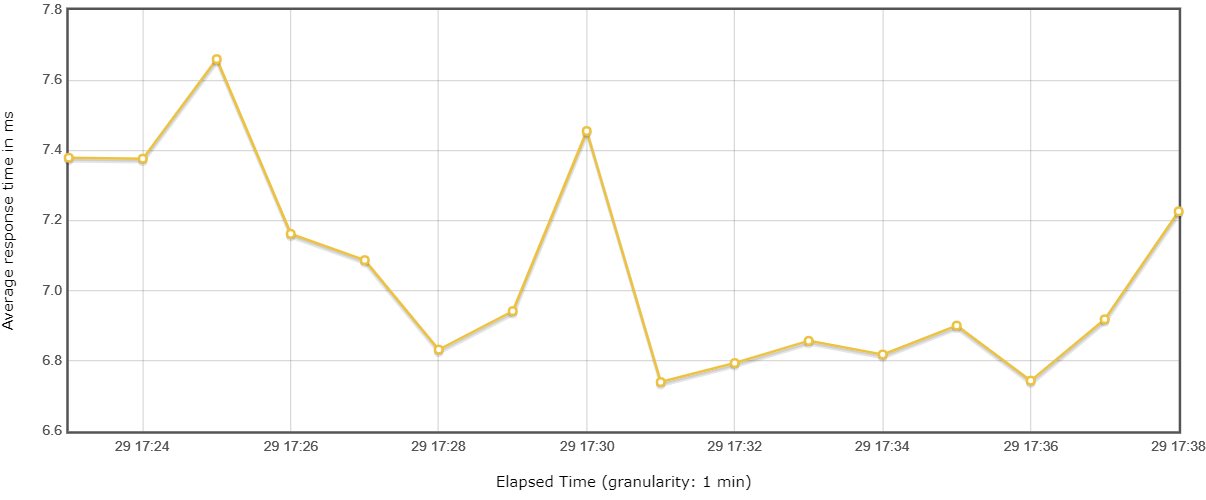
\includegraphics[width=1.0\textwidth]{gfx/flotResponseTimesOverTime.png}
  \caption{Response Time Graph von Lasttest von Ressource Server ohne OPA}
  \label{fig:chapter04:flotResponseTimesOverTime}
\end{figure}

In \autoref{fig:chapter04:flotResponseTimesOverTime} ist ein Diagramm dargestellt, das die durchschnittliche Response Time von dem Ressource Server ohne Open Policy Agent über den gesamten Zeitraum des Lasttests darstellt. Auf der x-Achse ist die Zeit und auf der y-Achse die durchschnittliche Response Time zu dem jeweiligen Zeitpunkt. Es ist zu sehen, dass die Response Time anfangs höher ausfällt und sie kontinuierlich sinkt, bis sie auf ungefähr dem gleichen Niveau verbleibt. Das könnte damit erklärt werden, dass jeder Thread zunächst eine Verbindung durch den 3-Way-Handshake mit dem Server aufbauen muss, welcher zusätzliche Zeit in Anspruch nimmt und sobald die Verbindung aufgebaut ist, ist die Response Time dann niedriger ist. Über den gesamten Zeitraum bewegen sich aber die Response Times im Bereich zwischen 7,8 Millisekunden und 6,6 Millisekunden. 

\begin{figure}[htbp]
  \centering
  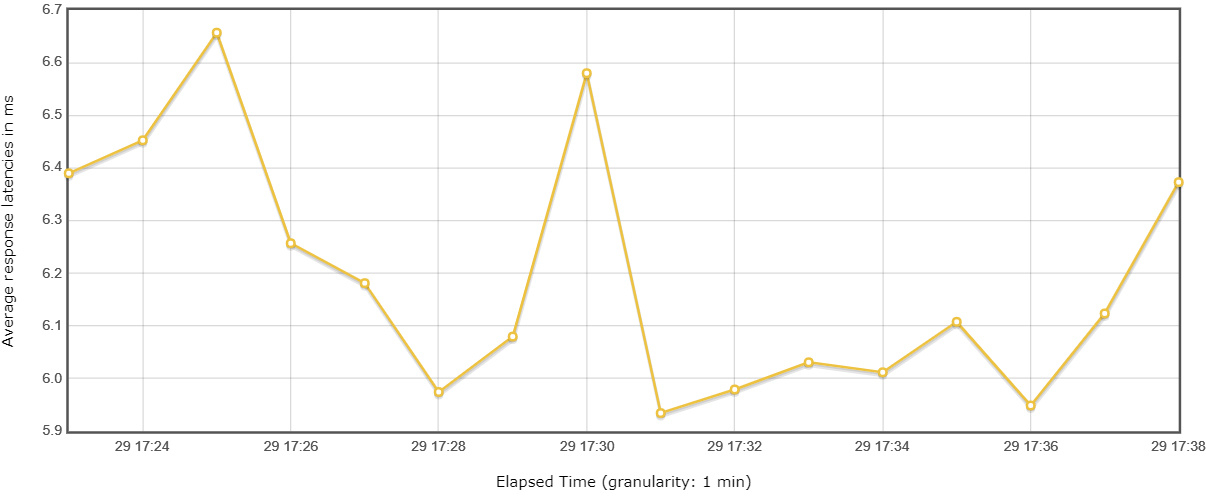
\includegraphics[width=1.0\textwidth]{gfx/flotLatenciesOverTime.png}
  \caption{Latency Time Graph von Lasttest von Ressource Server ohne OPA}
  \label{fig:chapter04:flotLatenciesOverTime}
\end{figure}

In \autoref{fig:chapter04:flotLatenciesOverTime} ist prinzipiell der gleiche Graph dargestellt, nur das hier anstatt der Response Time die Latenz dargestellt ist. Der Unterschied ist hier, wie in Kapitel 2.11 erläutert, dass die Latenz die Zeit vom bevor dem Senden der Anfrage bis zum Eintreffen des ersten Bytes der Antwort darstellt, während die Response Time die Zeit bis zum letzten Byte der Antwort misst. Die Latenz ist also immer kürzer als die Response Time. Hier ist zu sehen das zu dem Zeitpunkt 17:38 die Latenz 6,4 Millisekunden beträgt, während zum selben Zeitpunkt die Response Time 7,2 Millisekunden beträgt. In den folgenden Betrachtungen wird allerdings nur noch auf die Response Time eingegangen, da sie die wichtigere Metrik aus Nutzersicht ist, da ein Nutzer eine vollständige Antwort von dem Server haben möchte. Es ist keine zweckmäßige Beurteilung von Antwortzeiten möglich, wenn das erste Byte der Antwort des Servers zeitnah eintrifft, bis zum Eintreffen des letzten Bytes allerdings zwei Stunden vergehen. 

\begin{figure}[htbp]
  \centering
  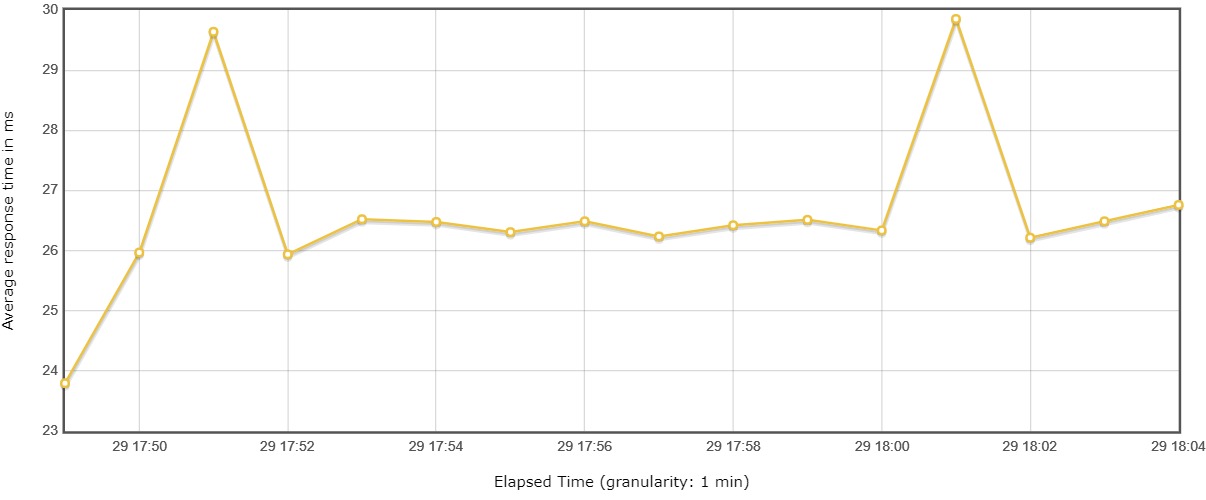
\includegraphics[width=1.0\textwidth]{gfx/flotResponseTimesOverTime-opa-last.png}
  \caption{Response Time Graph von Lasttest von Ressource Server mit OPA}
  \label{fig:chapter04:flotResponseTimesOverTime-opa-last}
\end{figure}

In \autoref{fig:chapter04:flotResponseTimesOverTime-opa-last} ist der Response Time Graph von dem Server dargestellt, der die Zugriffskontrolle mittels Open Policy Agent entkoppelt hat. Auch hier ist die Response Time anfangs höher, bis sie sich auf ein niedrigeres Level einpendelt. Aber das weitaus wichtigere ist, dass die Response Time hier durchschnittlich um ein Vielfaches höher ausfallen als bei dem Server mit interner Zugriffskontrolle. Die meiste Zeit über bewegen sich die Response Times hier zwischen 26 und 30 Millisekunden, während sie bei dem Server mit interner Zugriffskontrolle sich zwischen 6,4 und 7,2 Millisekunden bewegen.\smallskip

Dies ist insofern überraschend, da die Kommunikation, die zwischen Ressource Server und Open Policy Agent auftritt, auf localhost zu localhost Basis verläuft. Das heißt der Ressource Server und Open Policy Agent laufen auf derselben Maschine und es war nicht vorhersehbar, dass durch die http-Kommunikation zwischen diesen beide Komponente eine derart hohe zusätzliche Latenz entsteht. 
